\section{Definiciones básicas}
La termodinámica es la rama de la física encargada de comprender relaciones entre propiedades, que pueden no tener conexión alguna previo al análisis, sin dar una lógica causal.
De esa forma llega a poner límites a los procesos, en vez de explicar el proceso.
\begin{definition}[Sistema]
Toda región del universo dispuesta para el estudio del problema se denomina \emph{sistema}.
Todo el resto se denomina \emph{ambiente} o \emph{entorno}.
El borde del sistema se denomina \emph{contorno}; si este no permite el paso de materia se denomina \emph{abierto}, si no se denomina \emph{cerrado} (aunque esta definición es más amplia a la interacción de energía).
\end{definition}
\begin{definition}[Variables termodinámicas]
Son propiedades o magnitudes físicas necesarias para describir el proceso a estudiar.
Salvo la temperatura, la mayoría de estas magnitudes son de origen externo a la termodinámica.
La variables que dependan del tamaño del sistema se llaman \emph{extensivas}, que notamos en general como $X_i$, y las que no dependen del tamaño del sistema se llaman \emph{intensivas}, notadas como $X_i$.
\end{definition}
\begin{definition}[Estado] Habiendo definidas todas las variables termodinámica de un sistema decimos que el \emph{estado} del sistema está definido. \end{definition}
\begin{definition}[Equilibrio]
Un sistema está en equilibrio si y sólo si para cambiar el estado es necesario un cambio del ambiente, por lo que en el caso estacionario (que no hay flujos constantes de entrada y de salida) las variables se mantienen constantes.
Si el sistema está estacionario además no tiene información de cómo llegó el sistema a ese estado de equilibrio.
\end{definition}
La termodinámica podemos plantearla de varias formas posibles, nosotros vamos a mezclar algunas leyes con los postulados, pero solamente con los postulados es suficiente para formalizar toda la teoría física.
El primer postulado es necesario para darle sustento físico a la teoría, ya que a priori pueden no existir los estados de equilibrio
\begin{principle}[Existencia de los estados de equilibrio]
Existen los estados de equilibrio para sistemas caracterizados por finitas variables termodinámicas extensivas.
\end{principle}
La elección de variables termodinámicas de un sistema está sólamente condicionada por la experiencia física, por lo que es relevante para el sistema según el observador.
\begin{law}[Cero: Transitividad del equilibrio]
Si hay dos sistemas $A$ y $B$ en equilibrio térmico, es decir misma temperatura, y otro sistema $C$ está en equilibrio con $B$, entonces $A$ y $B$ están en equilibrio
\end{law}
\section{Primera Ley}
Joule en XXXX dispuso en una caja adiabática un líquido (uso agua, mercurio y otros materiales) con un método mecánico para revolverlo, como vemos en la figura \ref{fig:primera_ley}.
\begin{wrapfigure}{r}{0.35\linewidth}
\centering
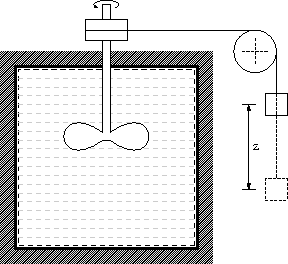
\includegraphics[width=0.35\textwidth]{primera_ley}
\caption{Experiencias de Joule}
\label{fig:primera_ley}
\end{wrapfigure}
La idea de la experiencia que el cuerpo cae a velocidad constante, por lo que toda la energía potencial se transfiere efectivamente al medio fluido (y como tiene una límite adiabático es la \emph{única} forma de alterar el sistema), y observar el cambio de temperatura del medio.
Joule observó que dicho cambio de temperatura sólo depende de la altura del cuerpo, es decir, de la energía potencial del cuerpo.
Además observó el mismo cambio de estado cambiando el mecanismo de ingreso de energía, por ejemplo por fricción o por una corriente eléctrica, o el sistema en si, un fluido diferente como el mercurio.
Es decir, Joule encontró que existe una magnitud conservativa (que sólo depende del estado inicial y final) independiente de la naturaleza del sistema que está asociada a la energía externa ingresante a dicho sistema, que llamamos \emph{energía interna} $U$
\begin{definition}[Energía interna]
La energía interna corresponde al trabajo adiabático efectuado en el sistema
\begin{equation}
dU = - d'W_{ad}
\end{equation}
La energía del sistema sólo depende del estado inicial y final, es decir
\begin{equation}
\oint dU = 0
\end{equation}
\end{definition}
Como ya mencionamos arriba, la energía $U$ es conservativa, así que debe existir una ley de conservación asociada.
Continuando con sus experiencias, Joule observó que la energía mecánica necesaria para llevar de un estado a otro sólo con transferencia de calor son equivalentes.
Es decir, Joule disponía de un cuerpo $B$ y otro $A$, con diferentes temperaturas, y al unirlos con una interface diatérmica hubo un cambio de estado; este cambio de estado corresponde a un valor de calor que es equivalente al trabajo necesario para llevar la temperatura del sistema que se enfrió a su temperatura al principio de la experiencia.
Con esta deducción Joule estableció la naturaleza del calor: es un tipo de energía
\begin{law}[Primera: Conservación de la energía]
El primer principio o postulado de la termodinámica determina que el trabajo efectuado en el sistema en condiciones adiabáticas sólo depende de las condiciones iniciales y finales, o dicho de otra manera, el trabajo entre dos estados de equilibrio es independiente del proceso efectuado (siempre en condiciones adiabáticas). En caso de tener una transformación no adiabática, la diferencia entre el trabajo efectuado y la energía interna es el calor
\begin{equation}
\Delta U = Q - W \Rightarrow dU = \delta Q - \delta W
\end{equation}
\end{law}
La diferencia entre $d$ y $\delta$ es que el trabajo y el calor si depende de la transformación, pero la energía interna no. En matemática los $d$ se llaman exactos, y verifican que sus magnitudes son conservativas.
\subsection{Trabajos generalizados}
La conservación de la energía no sólo funciona a sistemas simples, si no se ha encontrado sistema donde no se aplique. Pero para eso necesitamos generalizar el concepto de trabajo, usando el concepto de magnitud extensiva e intensiva
\begin{definition}[Variable extensiva e intesiva]
Una variable termodinámica extensiva $X$ corresponde a una magnitud que varia con el cambio del sistema, en general aumenta si aumenta el sistema, mientras una variable intensiva $Y$ no depende del tamaño del sistema.
\end{definition}
Ahora vamos a pasar a definir el trabajo generalizado, a partir del concepto de trabajo mecánico, que corresponde a $dW = F dx$, es decir el producto de una fuerza, que en el formalismo termodinámico corresponde a una variable intensiva, por un desplazamiento, una variable extensiva. De esta forma
\begin{definition}[Trabajo generalizado]
El trabajo \textit{de configuración} corresponde al trabajo necesario para llevar de un estado de equilibrio a otro estado de equilibrio de forma reversible, que se debe expresar como
\begin{equation}
d'W = \sum_i Y_i dX_i
\end{equation}
con $Y_i$ una variable intensiva y $X_i$ una variable extensiva
mientras que el trabajo \textit{disipativo} corresponde al efectuado de forma irreversible y no puede ser expresado con combinación lineal de diferenciales.
\end{definition}
Veremos que en concepto de trabajo de configuración podemos incluir el calor, cuando definamos la entropía.
Las variables que determinan un trabajo generalizado de configuración se denominan \emph{variables conjugadas}.
\section{Segunda ley}
En este principio, desarrollado antes que el primer principio históricamente, determina una imposibilidad de la naturaleza, además trae consigo una asimetrí temporal a los estados; determina la flecha del tiempo.
Pero ya vamos a ver todo eso.
Primero observemos el enunciado de Kelvin, que finalmente escribiremos como un postulado
\begin{law}[Enunciado de Kelvin]
No es posible tener una máquina térmica ciclica que tenga como único resultado eliminar calor de una fuente y transformarlo en trabajo.
\end{law}
De este principio nos queda definir que es una máquina térmica ciclica
\begin{definition}[Maquina térmica ciclica]
Proceso que altera el sistema desde un estado hasta otros estados, finalmente retornando al mismo estado inicial
\begin{figure}[H]
\centering
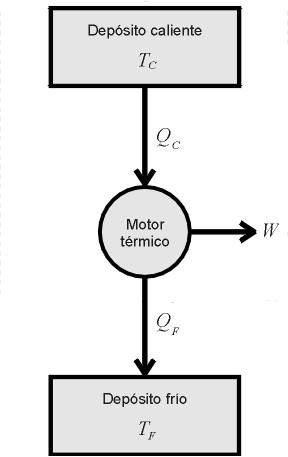
\includegraphics[width=0.18\textwidth]{motor}
\caption{Esquema simbólico del motor térmico}
\end{figure}
\end{definition}
El enunciado de Kelvin nos indica que la eficiencia de los motores no puede ser del 100\%, ya que
\begin{equation}
\eta = \frac{W}{Q_{in}} < 1
\end{equation}
\begin{collorary}[Existencia de la entropía]
Para todo sistema existe una función $S = S(U, \{X_i\})$, es decir función de las variables extensivas del sistema (en general $U$, $V$ y $N$), tal que una transformación isoentrópica reversible ($dS = 0$) implique que la transformación es además adiabática, es decir $dS = 0 \Leftrightarrow \delta Q = 0$.
Además de la definición se deduce que es una función de estado, ya que dado un estado tiene un valor definido independiente del camino ejecutado (a menos de una constante para todos los estados).
\end{collorary}
Para demostrar la existencia de la entropía, construimos un espacio dado por las variables extensivas $\{U,X_i\}$ (que vamos a tomar, para simplificar las ideas, $\{U,V,N\}$).
En ese espacio definimos un punto $A$, y otro $A'$ separados por una curva de $\{X_i\}$ constante.
Esos dos puntos están unidos por una curva no adiabática, es decir al tener diferente energía $U(A) \neq U(A')$, pero a $\{X_i\}$ constante, es necesario que ese cambio energético sea en forma de calor, es decir
\[U(A') = U(A) + Q_{A \to A'}.\]
Ahora si volvemos de $A'$ a $A$ por un camino adiabático, por lo que
\[U(A) = U(A') - W_{A' \to A},\]
pero efectuamos un ciclo cerrado donde transformamos calor en trabajo (ya que asumimos que pasar de $A$ a $A'$ implica agregar trabajo, es decir la curva es con $U$ creciente), siendo un proceso imposible según el enunciado de Kelvin.
Esto define conjuntos de puntos accesibles con procesos adiabáticos, que forman superficies que no se interfieren (por lo que ya vimos recién).
Un esquema de lo que efectuamos acá se presenta en la figura \ref{fig:segunda_ley_espacio}, pero considerando otros puntos del espacio.

\begin{figure}[H]
    \centering
    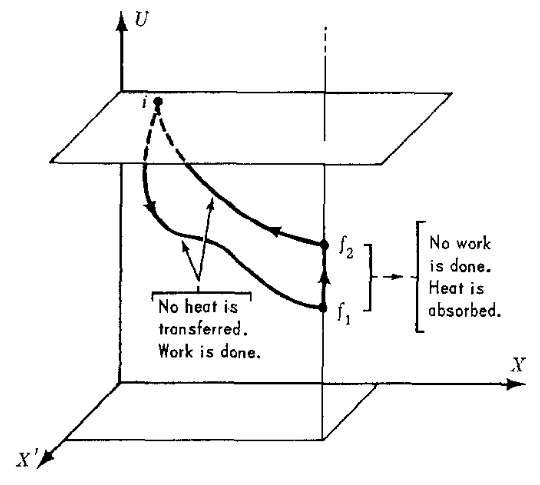
\includegraphics[width=0.6\textwidth]{segunda_ley_espacio}
    \caption{Diagrama del argumento para seleccionar puntos inalcanzables por transformaciones adiabáticas}
    \label{fig:segunda_ley_espacio}
\end{figure}

Esas superficies las vamos a parametrizar con \[S(U,\{X_i\}) = c,\] siendo S una función continua suave (ya que asumimos que las superficies son suaves), la \emph{entropía}.
Por definición, las superficies de nivel de $S(U,\{X_i\})$ son adiabáticas, y además podemos escribir a la energía como
\[dU = \frac{\partial U}{\partial S} dS + \frac{\partial U}{\partial X_i} dX_i = \delta Q - \delta W\]
de lo que se deduce automáticamente que el calor debe ser (ya que si $dS = 0$ entonces es necesario que $\delta Q = 0$)
\begin{equation}
\delta Q = \frac{\partial S}{\partial U} dS
\end{equation}
Si elegimos $\lambda = \frac{1}{T}$ a priori, podemos ver después que realmente es una temperatura, verificando la ley cero y la noción que tenemos de ella. Esto determina que
\begin{equation}
\frac{1}{T} = \left.\frac{\partial S}{\partial U}\right|_{X_i}
\end{equation}
\begin{collorary}[Desigualdad de Clausius]
Para una transformación cualquiera se verifica que \[T dS \geq \delta Q\] siendo una igualdad si el proceso es reversible
\end{collorary}
Para demostrar este colorario utilizamos nuevamente dos estados $A$ y $A'$ en el espacio $\{U,X_i\}$ unidos por una transformación (puede ser reversible o no).
En esta transformación hay un intercambio de calor $\delta Q$, y luego se genera una transformación adiabática a un estado nuevo $B$, conectado con $A$ por medio de una curva $\{X_i\}$ constante.
El calor en todo este ciclo es
\[\delta Q + \delta Q_{A' \to B} + \delta Q_{B \to A} = \delta Q + 0 - T dS.\]
Ese último despeje deriva que el proceso de $B$ a $A$ es reversible, por lo que $U(B) - U(A) = dU = T dS$, al ser las demás variables constantes. De Kelvin podemos deducir que el calor total debe ser negativo, ya que al haber calor positivo en el primer proceso y calor negativo en el segudo debió haber un trabajo positivo en el intermedio, por lo que finalmente se llega a que
\[\delta Q \leq T dS\]
para cualquier transformación.
Además podemos ver que $\lambda = \frac{1}{T}$, es factor integrante, es realmente una temperatura.
Para eso tomamos dos sistemas $1$ y $2$ en contacto térmico.
El sistema $1$ está a mayor temperatura que el sistema $2$. La entropía ya sabemos que es extensiva y aditiva (como la energía), por lo que
\[dS_{T} = dS_1 + dS_2 = -\frac{Q}{T_1} + \frac{Q}{T_2} = Q \left(\frac{1}{T_2} - \frac{1}{T_1}\right).\]
De la desigualdad de Clausius obtenemos que $T dS \geq 0$ por lo que para que la temperatura fluya de $1$ a $2$ se debe dar que $T_1 > T_2$.
Lo mismo podemos hacer para $T_2 > T_1$. Queda demostrado que el factor integrante es una temperatura, y además es imposible que se de el flujo de calor de otra forma, es decir
\begin{collorary}[Enunciado de Clausius]
No es posible mover con una máquina térmica cíclica calor de una fuente fría a una caliente, sin agregar trabajo.
\end{collorary}
con lo que cerramos los enunciados históricos de la segunda ley.
Nos queda deducir el teorema de Carnot para una máquina ciclica, que es fácil de deducir ya que sabemos que
\[\eta = \frac{W}{Q_{\in}} = \frac{Q_{in} - Q_{out}}{Q_{in}} = 1 - \frac{Q_{out}}{Q_{in}} \leq 1 - \frac{T_{f} \Delta S}{T_C \Delta S}\]
lo que finalmente se deduce en
\begin{collorary}[Teorema de Carnot]
El trabajo de cualquier máquina térmica, reversible o no, es menor igual a la unidad menos la relación entre la temperatura del reservorio frio y la del reservorio caliente\
\begin{equation}
\eta \leq 1 - \frac{T_F}{T_C}
\end{equation}
\end{collorary}
\section{Propiedades intensivas, relaciones}
Hemos asumido en los apartados anteriores que la energía y la entropía son funciones extensivas, por lo que son homogeneas de primer orden
\[ U(\lambda S, \{\lambda X_i \}) = \lambda U(S,\{X_i\}) \]
Si derivamos respecto a $\lambda$ de ambos términos
\[ \frac{\partial U(\lambda S, \{\lambda X_i\})}{\partial (\lambda S)} \frac{\partial (\lambda S)}{\partial \lambda} + \frac{\partial U(\lambda S, \{\lambda X_i\})}{\partial (\lambda X_i)} \frac{\partial (\lambda X_i)}{\partial \lambda} = U(S,\{X_i\})\]
Si evaluamos en $\lambda = 1$ como caso particular (por el cual no se pierde generalización), obtenemos la siguiente relación
\begin{equation}
U = T S + X_i Y_i
\label{eq:euler}
\end{equation}
donde sabemos que las variables intensivas conjugadas
\begin{equation}
Y_i = \left.\frac{\partial U}{\partial X_i}\right|_{T,X_j}
\end{equation}
La ecuación resultante se denomina ecuación de Euler.
Para la entropía podemos hacer el mismo proceso, obteniendo
\begin{equation}
S = \frac{U}{T} - \frac{Y_i}{T} X_i
\label{eq:euler_entropia}
\end{equation}
Si diferenciamos ambos términos de la ecuación de Euler, y simplificamos obtenemos la siguiente relación
\begin{equation}
S dT - X_i dY_i = 0
\label{eq:gibbs_durheim}
\end{equation}
llamada de Gibbs-Durheim, que nos permite relacionar las variables intensivas entre si.
La ecuación de Gibbs-Durheim impide la existencia de potenciales termodinámicos con variables intensivas solamente.
\section{Potenciales termodinámicos}
Ahora vamos a pasar a encontrar \emph{potenciales termodinámicos}, es decir funciones que en diferentes casos al ser minimizadas o maximizadas nos dan el estado de equilibrio.
Con esta definición ya es claro que la entropía $S = S(U,\{X_i\})$ es un potencial, pero respecto a variables no muy útiles experimentalmente.
También podemos encontrar lo mismo para la energía $U = U(S,\{X_i\})$, que debe ser un mínimo a respecto la entropía y las demás variables extensivas.
Nuevamente vemos que la energía interna así planteada no tiene utilidad experimental, ya que es muy complicado de medir la entropía (en general se la deduce).
Para eso usamos transformadas de Legendre
\subsection{Transformada de Legrendre}
Supongamos que tenemos una función de dos variables (se puede extender a cualquier cantidad de variables) $f(x,y)$ y una variable $z = \left.\dfrac{\partial f}{\partial x}\right|_y$.
Si quiero una función $\tilde{f}(z,y)$, la transformada de Legrende la define así
\begin{equation}
\tilde{f}(z,y) = f(x,y) - \left.\frac{\partial f}{\partial x}\right|_y x = f(x,y) - z\, x
\label{eq:legendre}
\end{equation}
Nos queda demostrar que las derivadas de la función nueva son lo que queremos que sea
\[\frac{\partial \tilde{f}}{\partial z} = \frac{\partial}{\partial z} \left( f(x(y,z),y) - x(y,z) \, z \right) = \frac{\partial f}{\partial x} \frac{\partial x(y,z)}{\partial z} - \frac{\partial x}{\partial z} z - x = z \frac{\partial x}{\partial y} - \frac{\partial x}{\partial y} z - x = - x.\]
La otra derivada la calculamos de la misma forma
\[\left.\frac{\partial \tilde{f}}{\partial y}\right|_z = \frac{\partial f}{\partial y} + \frac{\partial f}{\partial x} \frac{\partial x}{\partial y} - \frac{\partial x}{\partial y} z = \frac{\partial f}{\partial y}.\]
Estas dos relaciones las podemos unir en
\begin{equation}
\begin{gathered}
\left.\frac{\partial \tilde{f}(z,y)}{\partial z}\right|_y = - x\\
\left.\frac{\partial \tilde{f}(z,y)}{\partial y}\right|_z = \left.\frac{\partial f(x,y)}{\partial y}\right|_x
\end{gathered}
\end{equation}
El diferencial de la función $\tilde{f}$ es por lo tanto
\begin{equation}
d\tilde{f} = -x dz + \frac{\partial f}{\partial y} dy
\end{equation}
\subsection{Energias libres y entalpia}
Con la definición de transformación de Legandre, pasemos a encontrar algunas funciones derivadas de la energía $U = U(S,\{X_i\}$.
Para empezar encontremos una función $F = F(T,\{X_i\})$, es decir intercambiando entropía con temperatura, siendo una función más fácil de encontrar experimentalmente.
Sabemos que $T = \dfrac{\partial U}{\partial S}$, por lo que
\[ F(T,V,\{X_i\}) = U[T,V,\{X_i\}) U - S \frac{\partial U}{\partial S}\]
\begin{equation}
\begin{gathered}
F = U - T\,S \\
dF = - S\,dT - p d V - Y_i dX_i
\end{gathered}
\label{eq:energia_helmoltz}
\end{equation}
función que llamamos energía libre de Helmholtz.
Si trabajamos sobre el diferencial de la energía libre, usando la desigualdad de Clausius, tenemos que
\[dF = dU - T dS - SdT = (\delta Q - T dS) - \delta W - S dT \leq - \delta W - S dT\]
que para el caso de temperatura constante $dT = 0$ nos queda
\begin{equation}
dF \leq - \delta W
\end{equation}
es decir que el trabajo maximo extraíble a temperatura constante depende solamente de la energía libre, como bien su nombre describe.
El máximo se dará en el caso extraíble, donde $dF = - \delta W$
Además sin el trabajo es nulo, el estado de equilibrio se dará cuando
\begin{equation}
dF \leq 0
\end{equation}
es decir cuando sea un mínimo de la energía libre.
Por esto es que se denominan potenciales termodinámicos
Lo mismo podemos hacer con la presión y la tempratura, es decir
\begin{equation}
\begin{gathered}
G = U[T,p,\{X_i\}] = U - T\,S + p \, V \\
dG = S\,dT + V dp - X_i dY_i
\end{gathered}
\label{eq:energia_gibbs}
\end{equation}
Esta función se llama energía libre de Gibbs, o función de Gibss.
Esta función es en particular útil para transformaciones de fase, ya que ocurren a temperatura y presión constante, al menos en las fases "comunes".
Además si el trabajo generalizado es solamente
\[\delta W = p dV - \mu dN\]
entonces la energía libre de Gibbs a temperatura y presión constante es
\begin{equation}
G = \mu N
\end{equation}
Veamos el diferencial de esta función
\[dG = dU - T dS - S dT + p dV + V dp + X_i dY_i = (\delta Q - T dS) - (\delta W - p dV) - S dT + V dp + X_i dY_i \leq V dp - S dT - (\delta W - p dV\]
Si la temperatura y la presión son constantes entonces
\[dG \leq \delta W - p dV = p_{ext} dV - p dV = 0\]
donde asumimos que la transformación es cuasiestacionaria, por lo que finalmente deducimos que la energía libre de Gibbs es un mínimo, siendo un potencial termodinámico.
De forma general, cualquier función que sea una transformación de Legendre de la energía será minimo, en caso de que las variables acordes estén fijadas. Esto nos permite generar toda una familia de funciones, pero las más comunes ya las presentamos
Nos queda la entalpía, que corresponde a
\begin{equation}
\begin{gathered}
H = U[S, p, \{X_i\}] = U + p\,V\\
dH = T dS + V dp - Y_i dX_i
\end{gathered}
\label{eq:entalpia}
\end{equation}
Por medio del siguiente gráfico podemos recordar rápidamente estas ecuaciones
\begin{figure}
\centering
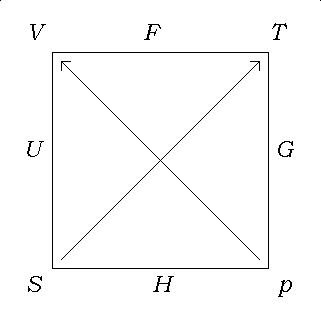
\includegraphics[width=0.5\textwidth]{potenciales}
\caption{Regla mnemotécnica para los potenciales termodinámicos}
\label{fig:potenciales}
\end{figure}
\subsection{Funciones de Massieu}
Las funciones de Massieu son las transformada de Legendre de la entropía, que podemos llamar entropías libres.
La primera es el potencial de Massieu
\begin{equation}
\begin{gathered}
\Phi = S[T,V,\{X_i\}] = S - \frac{U}{T}\\
d\Phi = -U d\frac{1}{T} + \frac{p}{T} dV + \frac{Y_i}{T} dX_i\\
d\Phi = \frac{U}{T^2} dT + \frac{p}{T} dV + \frac{Y_i}{T} dX_i
\end{gathered}
\end{equation}
Ese potencial lo podemos entender como
\begin{equation}
\Phi = - \frac{F}{T}
\end{equation}
Lo mismo podemos hacer con la energía libre de Gibbs, llamada entropía libre de Gibbs o potencial de Planck,
\begin{equation}
\begin{gathered}
\Xi = S[T,p,\{X_i\}] = S - \frac{U}{T} - \frac{p}{T} V = - \frac{G}{T} = \Phi - \frac{p}{T} V\\
d\Xi = -U d\frac{1}{T} - V d\frac{p}{T} + \frac{Y_i}{T} dX_i\\
d\Xi = \frac{U + p V}{T^2} dT - \frac{V}{T} dp + \frac{Y_i}{T} dY_i
\end{gathered}
\end{equation}
Estas funciones son útiles en mecánica estadística, ya que el logaritmo de la función de partición (por la constante de Boltzmann) es igual a la función de Massieu respectiva a la condición del sistema.
\section{Relaciones fundamentales}
En este apartado vamos a estudiar algunas consecuencias matemáticas de la teoría hasta ahora descripta.
Además vamos a considerar las funciones que debo tener de otras teorías para que la termodinámica funcione, una ecuación caracteristica o varias ecuaciones de estado y derivadas.
\subsection{Relaciones de Maxwell}
De la teoría de los diferenciales exactos podemos derivar que para cualquier función $f(x,y)$ con diferencial
\[df = \frac{\partial f}{\partial x} dx + \frac{\partial f}{\partial y} dy\]
se verifica que las derivadas segundas crusadas son iguales, es decir
\[\frac{\partial^2 f}{\partial x y} = \frac{\partial^2 f}{\partial y x}\]
Todo esto si el diferencial es exacto, es decir si
\[\oint df = 0\]
Podemos encontrar una relación por cada función de estado, que llamamos \emph{relaciones de Maxwell}.
\subsection{Relaciones materiales}
Definamos algunas propiedades materiales. El calor específico es igual la relación entre el cambio de temperatura y el calor entregado para ese cambio
\begin{equation}
C = \frac{\delta Q}{d T} = T \frac{dS}{dT}
\end{equation}
Si estamos a volumen constante, podemos encontrar que
\begin{equation}
C_v = \left.\frac{\partial U}{\partial T}\right|_V = T \left.\frac{\partial S}{\partial T}\right|_V
\label{eq:cv}
\end{equation}
Si la presión es constante $dp = 0$, debemos escribor $dV$ en función de la temperatura y la presión, encontrando
\[C_p = T \frac{dS}{dT} = T \frac{\partial S}{\partial T} + T \frac{\partial S}{\partial V} \frac{dV}{dT} = C_v + T \left.\frac{\partial S}{\partial V}\right|_T \left.\frac{\partial V}{\partial T}\right|_p\]
donde usamos una relación de Maxwell (de $dF$) para el segundo término
\[\left.\frac{\partial S}{\partial V}\right|_T = \left.\frac{\partial p}{\partial T}\right|_V\]
con lo que obtenemos
\[C_p = C_v + T \left.\frac{\partial p}{\partial T}\right|_V \left.\frac{\partial V}{\partial T}\right|_p = C_v + T V \alpha \left.\frac{\partial p}{\partial T}\right|_V\]
Ahí definimos el coeficiente de \emph{expansión térmica} como
\begin{equation}
\alpha = \frac{1}{V} \left.\frac{\partial V}{\partial T}\right|_p
\end{equation}
Para el último término usamos que $dV = 0$, ya que la derivada es a volumen constante, y de la expresión del diferencial $dV$ despejamos $\dfrac{dp}{dT}$, que es
\[ \left.\frac{\partial p}{\partial T}\right|_V = \frac{\partial_T V |_p}{\partial_p V|_T} = \frac{\alpha}{\beta_T}\]
donde se definió la \emph{compresibilidad isotérmica}
\begin{equation}
\beta_T = - \frac{1}{V} \left.\frac{\partial V}{\partial p}\right|_T
\end{equation}
con lo que finalmente nos queda
\begin{equation}
C_p = C_v + T V \frac{\alpha^2}{\beta_T}
\end{equation}
Si tenemos tres de las relaciones materiales podemos deducir las demás, en caso de tener una sola fase (si tenemos más fases, habrá tres por cada fase).
Y podemos a su vez conseguir una relación entre la compresibilidad isotérmica y la \emph{compresibilidad isoentrópica}
\begin{equation}
\beta_S = - \frac{1}{V} \left. \frac{\partial V}{\partial p}\right|_S
\end{equation}
que es
\begin{equation}
\beta_T = \beta_S + \frac{T V \alpha^2}{C_p}
\end{equation}
\subsection{Ecuaciones características}
Si experimentalmente o por otro método teórico encontramos uno de los potenciales respecto a sus variables naturales, la teoría de ecuaciones diferenciales exactos nos permite integrar sin ninguna necesidad de constantes de integración.
Sin embargo, si no tenemos el potencial en sus variables naturales, tendremos el problema de las constantes de integración, que se transforman en funciones desconocidas.
Por ejemplo si tenemos la función $F(T,V,\{X_i\})$ en sus variables, podemos encontrar
\begin{equation}
\begin{gathered}
p = - \left.\frac{\partial F}{\partial V}\right|_{T}\\
S = - \left.\frac{\partial F}{\partial T}\right|_{V}\\
\end{gathered}
\end{equation}
y las relaciones de Maxwell acordes
\begin{equation}
\left.\frac{\partial p}{\partial T}\right|_V = \left.\frac{\partial S}{\partial V}\right|_T
\end{equation}
Además sabemos que $U = F + TS$, se tiene
\begin{equation}
C_v = \left.\frac{\partial U}{\partial T}\right|_V = T \left.\frac{\partial^2 F}{\partial T^2}\right|_V
\end{equation}
Lo mismo podemos hacer para los demás potenciales
\begin{equation}
\begin{gathered}
S = - \left.\frac{\partial G}{\partial T}\right|_p\\
V = \left.\frac{\partial G}{\partial p}\right|_T\\
\frac{\partial S}{\partial V} = \frac{\partial V}{\partial T}\\
C_p = -T \frac{\partial^2 G}{\partial T^2}\\
\beta_T = - \frac{1}{V} \frac{\partial^2 G}{\partial p^2}
\end{gathered}
\end{equation}
\begin{equation}
\begin{gathered}
T = \left.\frac{\partial H}{\partial T}\right|_p\\
V = \left.\frac{\partial H}{\partial p}\right|_T\\
\left.\frac{\partial V}{\partial S}\right|_p = \left.\frac{\partial T}{\partial p}\right|_S\\
\beta_S = - \frac{1}{V} \frac{\partial^2 H}{\partial p^2}
\end{gathered}
\end{equation}
\subsection{Ecuaciones de estado}
Una ecuación de estado se llama a una relación
\begin{equation}
Y_i = Y_i(\{X_j\})
\end{equation}
es decir una variable intensiva en función de las extensivas.
Ejemplos de eso puede ser
\[p = p(U,V) = p(S,V)\]
\[T = T(S,V) = T(U,V)\]
En general para gases tenemos que
\[p = p(T,V,N)\]
donde eliminamos $S$ por $T$ usando una transformación de Legendre.
Tener una ecuación de estado no te da toda la información termodinámica, pero teniendo todas las posibles para un sistema es equivalente a tener una ecuación característica, o tener las tres propiedades materiales necesarias por fase.
Si tenemos $r$ componentes, hay $r + 2$ ecuaciones (asumiendo que no hay más parámetros extensivos que $S$, $V$ y $N_i$), que nos dan toda las información del sistema.
Pero de la relación de Gibbs-Durheim podemos eliminar una ecuación, obteniendo $r + 1$ grados de libertad (que se corresponde con las variables intensivas independientes).
\section{Equilibrio}
En este apartado vamos a estudiar las propiedades en el equilibrio, sea térmico, mecánico o de otra especie.
Para eso usamos que la entropía es extremal, en particular máxima, para dos sistemas $1$ y $2$, y además que es aditiva
\[ dS_T = dS_1 + dS_2 = \frac{\partial S_1}{\partial X^1_i} dX^1_i + \frac{\partial S_2}{\partial X^2_i} dX^2_i \geq 0\]
Consideremos transformaciones cuasiestacionarias, así tenemos definido en todo el proceso las variables (en caso de no ser transformaciones reversibles, siempre podemos construirnos una tranformación intermedia reversible, si sabemos el estado inicial y final).
Esto último determina que la desigualdad es una igualdad
\[\frac{\partial S_1}{\partial X^1_i} dX^1_i + \frac{\partial S_2}{\partial X^2_i} dX^2_i = 0\]
El cambio de una magnitud extensiva en un sistema es menos el cambio de la otra, y para convencernos de eso pensemos en la energía y la cantidad de partículas, o el volumen si hay un pistón movil entre los dos sistemas.
Eso nos lleva a concluir que
\begin{equation}
\frac{\partial S}{\partial X^1_i} = \frac{\partial S}{\partial X^2_i}
\end{equation}
que para substancias definidas por $T$, $p$ y $\mu$ indica que
\begin{equation}
\begin{gathered}
T_1 = T_2 \\
p_1 = p_2 \\
\mu_1 = \mu_2
\end{gathered}
\end{equation}
que son el equilibrio térmico, mecánico y químico respectivamente.
\subsection{Estabilidad}
En todo el análisis anterior usamos que la entropía es un extremo, pero nos falta observar que implica que además sea un máximo.
En general la forma del extremo determina la \emph{estabilidad} del sistema, y en este caso como es un máximo de entropía, y por lo tanto un mínimo de energía, los equilibrios van a ser \emph{estables}.
Como ya vimos el máximo de la entropía se escribe
\[d^2 S \leq 0\]
que implica que la función debe ser concava en un entorno del equilibrio.
De la teoría del análisis multifuncional sabemos que el desarrollo de Taylor a orden 2 corresponde a
\[ f(\textbf{x}) = f(\textbf{x}_0) + Df(\textbf{x}_0) (\textbf{x} - \textbf{x}_0) + (\textbf{x} - \textbf{x}_0)^{T} Hf(\textbf{x}_0) (\textbf{x} - \textbf{x}_0) + R(f, \textbf{x},\textbf{x}_0)\]
donde el primer orden dispone del diferencial o jacobiano de la función y el segundo orden corresponde al hessiano (que podemos pensar como un tensor de rango 2), más el resto de Taylor (que para funciones analíticas es simplemente seguir escribiendo ordenes superiores, que podemos pensar como tensores).
Si la función $f(\textbf{x})$ tiene un extremo el teorema de Taylor nos determina la positividad del hessiano.
Para un máximo el hessiano debe ser definido negativo, y para un mínimo debe ser definido positivo.
El criterio de Sylvester nos indica que una matriz es definida positiva si todos los menores tienen determinantes positivos, o definida positiva si todos los menores con dimensión k pares son negativos y los impares positivos.
En caso de al entropía, que es una función $S(U,V,\{X_i\})$, sabemos que debe ser máxima en el equilibrio, por lo que usando el criterio de Sylvester se llega a que
\begin{equation}
\begin{gathered}
\left.\frac{\partial^2 S}{\partial U^2}\right|_{V,X_i} \leq 0 \qquad
\left.\frac{\partial^2 S}{\partial V^2}\right|_{U,X_i} \leq 0\\
\frac{\partial^2 S}{\partial U^2} \frac{\partial^2 S}{\partial V^2} - \left(\frac{\partial^2 S}{\partial U \partial V}\right)^2 \geq 0
\end{gathered}
\end{equation}
Para más variables se extrapola de forma análoga, pensando en el criterio propuesto.
La primera relación la podemos escribir
\[\left.\frac{\partial^2 S}{\partial U^2}\right|_V = - \frac{1}{T^2} \left.\frac{\partial T}{\partial U}\right|_V = - \frac{1}{T^2 C_v} \leq 0\]
lo que nos lleva a
\begin{equation}
C_v \geq 0
\end{equation}
Para continuar nos conviene ver la energía $U$, que sabemos que debe ser un mínimo, es decir
\begin{equation}
\begin{gathered}
\frac{\partial^2 U}{\partial S^2} = \left.\frac{\partial T}{\partial S}\right|_V \geq 0 \qquad
\frac{\partial^2 U}{\partial V^2} = - \left.\frac{\partial P}{\partial V}\right|_S \geq 0\\
\frac{\partial^2 U}{\partial S^2} \frac{\partial^2 U}{\partial V^2} - \left(\frac{\partial U}{\partial S \partial V}\right)^2 \geq 0
\end{gathered}
\end{equation}
Para los potenciales podemos hacer el mismo proceso, recordando el cambio de signo de la variable que cambiamos, por lo que si para la energía respecto a la entropía es un minimo, el potencial respecto a la temperatura será un máximo.
\begin{equation}
\left.\frac{\partial^2 F}{\partial^2 T}\right. = \left.\frac{\partial S}{\partial V}\right|_V \leq 0 \qquad
\left. \frac{\partial^2 F}{\partial^2 V}\right. = \left.\frac{\partial p}{\partial V}\right|_T \geq 0
\end{equation}
\begin{equation}
\left.\frac{\partial^2 G}{\partial T^2}\right. = \left.\frac{\partial S}{\partial T}\right|_p \leq 0 \qquad
\left.\frac{\partial^2 G}{\partial p^2}\right. = \left.\frac{\partial V}{\partial p}\right|_T \leq 0
\end{equation}
\begin{equation}
\left.\frac{\partial^2 H}{\partial S^2}\right. = \left.\frac{\partial T}{\partial S}\right|_p \geq 0 \qquad
\left.\frac{\partial^2 H}{\partial p^2}\right. = \left.\frac{\partial V}{\partial p}\right|_S \leq 0
\end{equation}
De estas expresiones podemos deducir las condiciones para las propiedades materiales
\begin{equation}
\begin{gathered}
C_{V,p} \geq 0\\
\beta_{T,S} \geq 0\\
\alpha_{P,V} \geq 0
\end{gathered}
\end{equation}
Pero además si consideramos la siguiente idéntidad
\begin{equation}
\frac{\beta_S}{\beta_T} = \frac{C_V}{C_p}
\end{equation}
encontramos que
\begin{equation}
\beta_T \geq \beta_S \geq 0 \qquad C_p \geq C_V \geq 0
\end{equation}
Recordemos que todas estas igualdades encontradas en este apartado son propias de los estados de equilibrio estables.
Pueden no verificarse en equilibrios inestables o metaestables, como vamos a ver en el apartado de cambio de fases.
\subsection{Principio de Le Chatelier}
Este principio dictamina que cualquier inhomogeneadad de un sistema en equilibrio tenderá al sistema a otro nuevo equilibrio, volviendo a la homogeneidad.
Esto lo podemos deducir sabiendo que las relaciones materiales son positivas, ya que si agregamos calor al sistema o si lo comprimimos, la fluctuación se va esparciendo en virtud de la positividad de las constantes.
Pero también podemos deducir que el comportamiento del sistema frente a fluctuaciones de un parámetro intensivo $X^f$ cualquiera; el subscripto indica que es una fluctuación.
Para eso, tomemos dos subsistemas $1$ y $2$, tal que el sistema esté aislado.
El cambio del parámetro $Y$ del sistema $1$ va a ser
\[dY^f_2 = \frac{\partial Y_1}{\partial X_1} dX^f_1\]
además que altera al sistema $2$
\[ dY^f_2 = \frac{\partial Y_2}{\partial X_1} dX^f_1\]
Hasta ahora definimos los cambios debido a las fluctuaciones.
Pasemos a describir el cambio de la energía debido a las respuestas, que señalaremos con un superindice $r$
\[d(U + U^r) = (Y_1 - Y^r_1) dX^r_1 + (Y_2 - Y^r_2) dX^r_2 \leq 0 \]
donde usamos que la energía debe ser un mínimo.
La expresión de arriba puede llevar finalmente a
\[ d(U + U^r) = dY^f_1 dX^r_1 + dY^f_2 dX^r_2 \leq 0\]
Como los diferenciales son independientes, tenemos que
\[dY^f_1 dX^r_1 = \frac{\partial Y_1}{\partial X_1} dX^f_1 dX^r_1 \leq 0\]
\[dY^f_2 dX^r_2 = \frac{\partial Y_2}{\partial X_1} dX^f_1 dX^r_2 \leq 0\]
La primera desigualdad nos indica que
\begin{equation}
dX^f_1 dX^r_1 \leq 0
\end{equation}
La respuesta de la variable intensiva es contraria a la fluctuación, es decir el principio de Le Chatelieur.
La segunda desigualdad la podemos trabajar usando una relación de Maxwell derivada de la energía
\[ \frac{\partial Y_2}{\partial X_1} = \frac{\partial Y_1}{\partial X_2}\]
en la forma
\[dX^f_1 \frac{\partial Y_1}{\partial X^2} dX^r_2 \leq 0.\]
Si multiplicamos a ambos lados por $\partial_{X_1} Y_1$ que sabemos que es positiva obtenemos
\[\frac{\partial Y_1}{\partial X_1} dX^f_1 \frac{\partial Y_1}{\partial X_2} dX^r_2 \leq 0\]
que es lo mismo que
\begin{equation}
dY^f_1 dY^r_1 \leq 0
\end{equation}
Nuevamente encontramos que la fluctuación del parámetro intensivo genera una respuesta contraria, en línea con el principio de Le Chatelieur.
\section{Cambio de fases}
En este apartado vamos a discutir el equilibrio y transición de fase
Toda transición de fase está caracterizada por una perdida de estabilidad de la substancia analizada en el sistema.
La fluctuaciones se encargaran de que la substancia esté en una fase u otra.
Las transiciones de fase se clasifican en \emph{primer orden} y \emph{segundo orden}, la primera tiene un calor latente y la segunda en general se llaman transiciones continuas, caracterizadas por una suceptibilidad (derivada segunda de la ecuación caracteristica) divergente.
Las transiciones de primer orden tienen además la particularidad de estar caracterizadas por la existencia de dos mínimos del potencial, separados por una barrera, mientras que las de segundo orden suceden en un sólo punto del espacio de configuraciones termodinámico (y por ello se denominan \emph{fenómenos críticos}).
Para las transiciones de primer orden podemos definir al calor latente como
\begin{equation}
l = T \Delta s
\end{equation}
siendo $\Delta s$ la diferencia de entropía molar entre las fases.
Como estamos hablando de una transiciones que ocurren a temperatura constante (y las fluctuaciones son debidas a alguna otra variable), trabajaremos con las energías libres.
En esas energías libres se observa la existencia de dos mínimos, uno más estable que otro (a menor energía libre, más estable).
Como la transición se efectúa a temperatura constante, debe haber un cambio de entropía (que lo tratamos de forma molar, para eliminarnos la cantidad de materia).
\subsection{Coexistencia de fases}
En los diagramas termodinámicos podemos encontrar curvas de coexistencia de fase, usando que como es un equilibrio entre dos especies.
Es decir
\[\mu_{1} = \mu_{2}\]
que es igual a la energía libre de Gibbs por mol de cada fase.
Tratarermos coexistencia de fases con presión y temperatura, ya que los casos que nos preocupan hay variaciones importantes de volumen molar.
Elijamos dos estados $A$ y $A'$ sobre la curva de coexistencia, pero de diferentes fases, lo mismo con $B$ y $B'$.
La diferencia de presión entre $A$ y $B$ la consideramos
\[p_B - p_A = dP\]
y lo mismo para la temperatura
\[T_B - T_A = dT\]
La curva de coexistencia tiene de pendiente $dp/dT$ en un diagrama $p-T$
Como estoy en un equilibrio de fases
\[\mu_A = \mu_A' \qquad \mu_B = \mu_B'\]
por lo que
\[\mu_B - \mu_A = \mu_B' - \mu_A'\]
y usando que $\mu$ es la energía libre por mol
\[\mu_B - \mu_A = -s dT + v dp = \mu_B' - \mu_A' = -s' dT + v' dp\]
de lo que deducimos finalmente
\begin{equation}
\frac{dp}{dT} = \frac{s' - s}{v' - v} = \frac{\Delta s}{\Delta v} = \frac{l}{T \Delta v}
\label{eq:clausius_clayperon}
\end{equation}
Esta es la ecuación de Clayperon, que determina la pendiente de las curvas de coexistencia, y además tiene embuido el principio de Le Chatelieur.
\[d\mu = \frac{V} dp + S dT\]
Como ya dijimos vamos a trabajar con presión y temperatura, pero en particular vamos a buscar cambios de fases a temperatura constante.
\subsection{Isotermas inestables}
Aunque las transiciones de primer orden las podemos entender como la existencia de varios minimos en la energía libre, podemos también encontrar casos de isotermas inestables, en particular en un diagrama $p-V$.
A saber, la segunda ley determina que
\[ \frac{\partial p}{\partial V}_T \leq 0\]
que en algunas ecuaciones de estado para gases no se cumple.
En general el proceso ocurre debido a que la ecuación de estado está derivada de ciertas hipótesis mecánicas sobre la substacia, como ser el gas ideal o de Van Der Waals, pero que algunas de las hipótesis se violan en la inestabilidad.
Al haber un estado inestable, y tener un cambio de fases gas a líquido, se pierde la hipótesis de homogeneadad, por lo que esa parte de la ecuación fundamental (o de estado) debe ser \emph{arreglada}.
Como estamos en un cambio de fases, debemos considerar el potencial químico entre dos estados sobre la isoterma, el cual podemos calcular por medio de la relación de Gibbs Durheim
\begin{equation}
\mu_B - \mu_A = \int^B_A v dP
\label{eq:isoterma_eq_fase}
\end{equation}
donde la constante de integración dependiente de la temperatura se eliminó al calcular variaciones del potencial químico.
Definido el potencial químico, la energía libre de Gibbs molar, y sabiendo que la presión en función del volumen tiene derivada positiva en algún intervalo, podemos deducir que el volumen respecto a la presión va a ser una función multivaluada.
De esta forma al integrar el volumen, la energía libre también será multivaluada, llevando a una contradicción.
Para salvar la contradicción, exigimos que el potencial químico en todo ese intervalo sea constante, propio de una curva de coexistencia de fases, por lo que la integral de \ref{eq:isoterma_eq_fase} esa nula
\begin{equation}
\int^B_A v dp = 0
\label{eq:regla_maxwell}
\end{equation}
que se llama regla de Maxwell, que para una isoterma oscilante exige areas iguales.
Para un gas de Van der Waals la forma de la curva de coexistencia será una recta horizontal generando areas iguales.
Recién cuando truncamos la isoterma con la regla de Maxwell tenemos una curva físicamente posible.
Esa curva crea un cambio brusco de $v(p)$, del volumen molar, por lo que también produce un cambio brusco de la entropía molar.
Como la entropía es una función de estado podemos integrarla con
\[ \Delta s = \int \left.\frac{\partial s}{\partial v}\right|_T dv = \int \left.\frac{\partial p}{\partial T}\right|_V dv\]
sobre la curva ficticia.
En cambio de entropía corresponde a un calor latente intercambiado.
Esto conlleva también un cambio de la energía interna molar, ya que
\[ \Delta u = T \Delta s - p \Delta v\]
Si unimos los extremos de las rectas de coexistencia según la regla de Maxwell obtenemos una curva tipo parabóla, que separa el diagrama $p-v$ en dos fases, gaseosa y líquido más gas.
La fracción de gas y líquido en la zona de coexistencia viene dado por la regla de la palanca, que corresponde a asumir que existe una sóla substancia con volumen $V = N v$, divida en dos subsistemas con volumenes $V_G = N x_g v_G$ y $V_L = N x_L v_L$, siendo $x_i$ la fracción molar ($\sum x_i = 1$).
Finalmente la regla queda
\begin{equation}
x_L = \frac{v_G - v}{v_g - v_L} = 1 - x_G
\end{equation}
La inestabilidad de un potencial genérico en función de sus variables $X_j$ lo podemos corregir uniendo con una línea recta los dos mínimos separados por una barrera, como vemos en la figura \ref{fig:fase_potencial}
\begin{figure}[H]
\centering
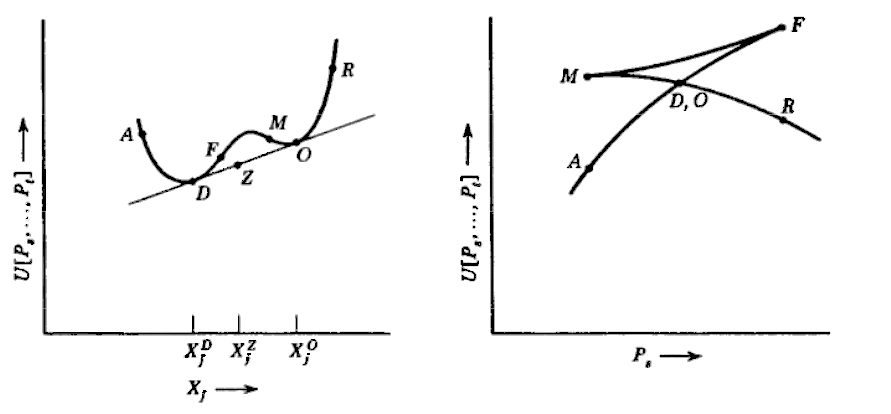
\includegraphics[width=0.5\textwidth]{fase_potencial}
\caption{Potencial generalizado en un caso de perdida de estabilidad, además de la correción con el método de Maxwell}
\label{fig:fase_potencial}
\end{figure}
La línea entre $D$ y $O$ se consigue exiguiendo potencial químico constante, como ya hicimos previamente para el caso isotérmico con el potencial de Gibbs..
\subsection{Regla de las fases de Gibbs}
Imaginemos que tenemos $R$ componentes en un equilibrio de fase.
Ya sabemos $R$ componentes diferentes implica que haya $R + 1$ variables
Consideremos que hay $N$ fases, por lo que las variables independientes de cada potencial químico van a ser $2 + M(r - 1)$ ($T$, $p$ y las fracciones molares).
Pero a su vez existen $r(M - 1)$ ecuaciones dadas por el equilibrio de fase, que corresponde a la igualdad entre potenciales químicos.
Esto nos dice que los grados de libertad que vamos a tener son
\begin{equation}
f = 2 + M(r - 1) - r(M - 1) = r - M + 2
\label{eq:regla_gibbs_fase}
\end{equation}
ecuación que se denomina regla de Gibbs de las fases.
De ahí podemos deducir que si tenemos un sólo componente, el punto triple no tiene grados de libertado posibles, por lo que es un único estado y además si hay dos fases para una componente tenemos una curva donde hay un sólo grado de libertad.
Si se tiene más grados se pasará a tener una superficie de coexistencia de fases.
\section{Tercer principio}
Un agregado final debido a Nerst, que se puede entender solamente en el contexto de la mecánica cuántica, es la tercera ley de la Termodinámica
\begin{law}[Mínimo de la entropía]
La entropía de un sistema tiende a una constante positiva al hacer nula la temperatura. Es decir
\[\displaystyle\lim_{T \to 0} S = S_0 \geq 0\]
Este valor corresponde al mínimo de entropía.
\end{law}
De esta ley, junto con la segunda ley, podemos deducir que no es posible alcanzar la temperatura $T = 0$ llamado cero absoluto.
La constante positiva podemos entenderla como la entropía remanente, debido a la degeneración del estado fundamental, que sólo se puede comprender entiendiendo la cuántica.
\section{Gases reales e ideales}
En este apartado vamos a presentar algunas ecuaciones de estado para gases, ideal o real, derivadas de principios básicos de la mecánica estadística.

\subsection{Gas ideal}
Podemos deducir de algunos resultados experimentales o simplemente deduciendola de la mecánica estadística: para un gas ideal, es decir sin interacciones entre partículas tenemos que
\begin{equation}
p V = n R T
    \label{eq:gas_ideal_estado}
\end{equation}
que corresponde al una ecuación de estado $p = p(V, n, T)$, con $n$ la cantidad de moles de substacia.
De esta forma la transformaciones isocóricas y isométricas son triviales, mientras que las transformaciones isotérmicas
\begin{equation}
    p = \frac{T}{v}
\end{equation}
son hipérboles en el plano $p-V$, como se ve en la figura \ref{fig:gas_ideal_isotermas}.
\begin{figure}[H]
    \centering
    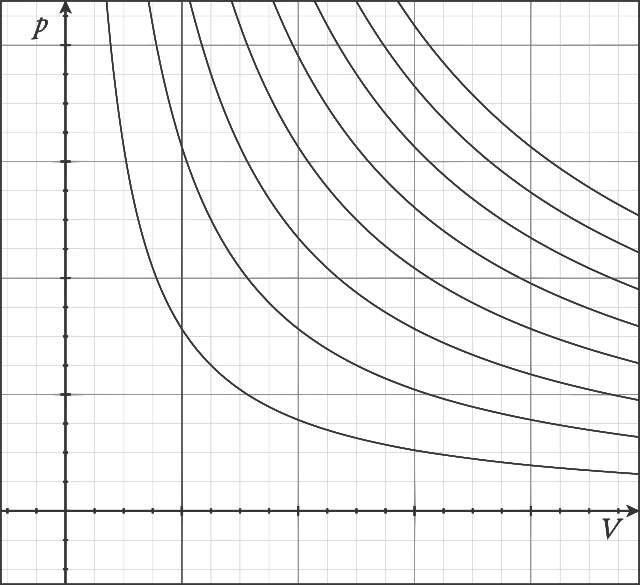
\includegraphics[width=0.4\textwidth]{gas_ideal_isotermas}
    \caption{Isotermas de un gas ideal con unidades arbitrarias}
    \label{fig:gas_ideal_isotermas}
\end{figure}

Interesante es que debido a la ecuación de estado, la energía $U$ no depende del volumen, ya que si tomamos el diferencial de entroía 
\[  dS = \left.\frac{\partial S}{\partial T}\right|_V dT + \left.\frac{\partial U}{\partial V}\right|_T dV\]
y lo reemplazo en la expresión de la primera/segunda ley
\[ dU = T \left.\frac{\partial S}{\partial T}\right|_V dT + \left( T \left.\frac{\partial S}{\partial V}\right|_T - p \right) = C_v dT + \left( T \left.\frac{\partial p}{\partial T}\right|_V - p \right) = C_v dT \]
es decir que la energía interna para un gas ideal es simplemente
\begin{equation}
    dU = C_v dT
    \label{eq:gas_ideal_energia}
\end{equation}

Experimentalmente (y de la mecánica estadística) se encuentra que el calor específico es constante con la temperatura y que además vale
\begin{equation}
    C_v = \frac{3}{2} N k_B
    \label{eq:gas_ideal_cv}
\end{equation}
Con esto tenemos el gas ideal caracterizado, porque podemos deducir la energía interna
\begin{equation}
    U = \frac{3}{2} N k_B T
\end{equation}
donde aparece la \emph{equipartición de la energía} en forma de tres grados de libertad con $\frac{N k_B T}{2}$ energía, y también podemos encontrar la entropía
\begin{equation}
    S = C_v \ln\left(\frac{T}{T_0}\right) + N K \ln\left(\frac{V}{V_0}\right)
\end{equation}
A partir de la expresión de la entropía podemos deducir la funciona de una transformación adiabática, usando que la entropía $S = cte$,

\begin{equation}
    V T^{\frac{C_v}{N k_B}} = c \qquad T V^{\frac{N k_B}{C_v}} = c
\end{equation}
que se puede llevar a
\begin{equation}
    p V^{1 + \frac{C_v}{N k_B}} = p V^{\frac{C_v + N k_B}{C_v}} = p V^{\gamma} = c
\end{equation}
donde también podemos deducir que
\begin{equation}
    C_p - C_v = N k_B
\end{equation}
por lo que 
\begin{equation}
    \gamma = \frac{C_p}{C_v}
\end{equation}
que para un gas ideal monoatómico es igual a $\gamma \dfrac{3}{2}$.
Esa relación la diferencia de una isoterma, que sería de la forma de una adiabática pero con $\gamma = 1$, que sólo es posible de obtener si el gas tiene 2 grados de libertad (como un gas en dos dimensiones).

\subsection{Gas de Van der Waals}

La primer teoría exitosa de los gases reales fue la propuesta por Van Der Waals, proponiendo la existencia del volumen excluido, que corresponde al volumen de cada partícula de gas, y a la iteracción por choques entre partículas, que trató a primer orden.
De esta forma llegamos a que 
\begin{equation}
\left(p + \frac{a N^2}{V^2}\right)(V- b N) = N k_B T
\label{eq:vanderwalls}
\end{equation}
que podemos escribir de la siguiente forma
\begin{equation}
p = \frac{R T}{v - b} - \frac{a}{v^2}
\label{eq:vanderwalls_intensivo}
\end{equation}
La ecuación de Van der Waals es exitosa en describir cualitativamente el comportamiento de los gases reales, sin producir comportamientos físicamente absurdos, pero cuantitavamente varía mucho dependiendo de la elección de los parámetros $b$ y $a$.

Veamos las isotermas, que las graficamos en la figura \ref{fig:gases_vdw_isotermas}
\begin{figure}[H]
    \centering
    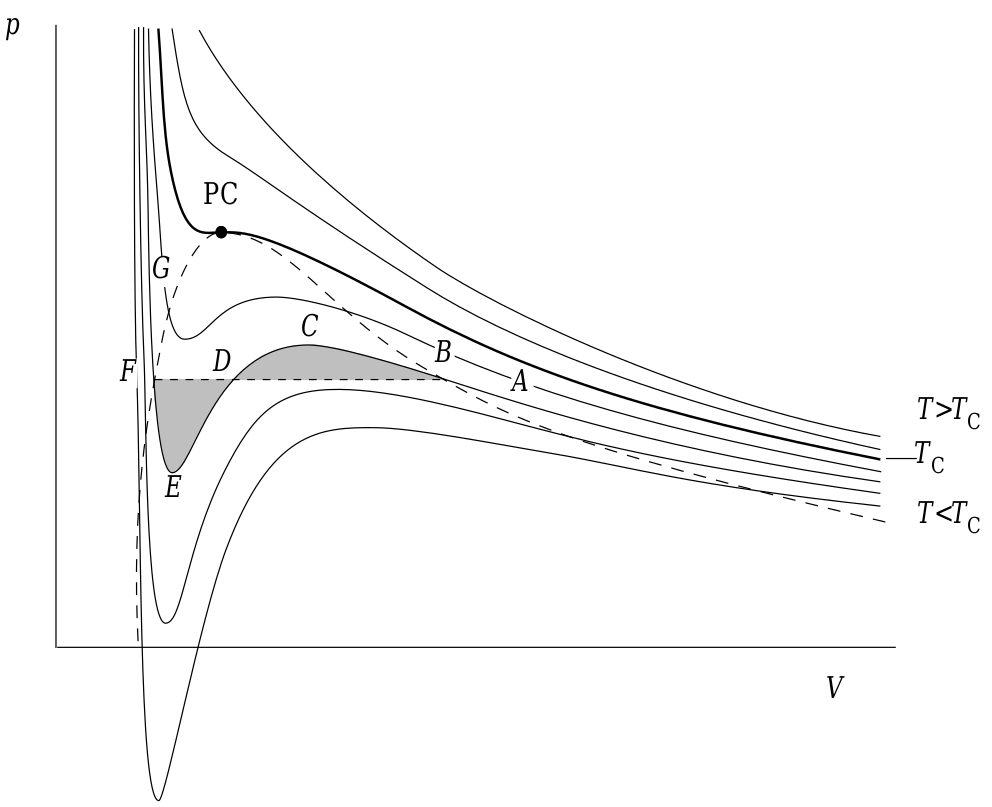
\includegraphics[width=0.5\textwidth]{gases_vdw_isotermas}
    \caption{Diagrama p-V con isotermas, adimensionalizadas, del gase de Van der Waals, más el punto crítico y la zona de coexistencia}
    \label{fig:gases_vdw_isotermas}
\end{figure}

En esa figura se observa que dentro de la zona demarcada por la curva punteada existe una oscilación que no tiene correlato físico, ya que es inestable.
En esa zona se produce un cambio de fase, y se arregla con la regla de Maxwell, recta que está marcada con el sombreado en una de las oscilaciones.

Mientras el punto crítico nos permite definir una temperatura, volumen y presión y adimensionalizar la ecuación de Van der Waals.
En el punto crítico tenemos que

\begin{equation}
    \left.\frac{\partial p}{\partial V}\right|_{T_c} = 0 \qquad \left.\frac{\partial^2 p}{\partial V^2}\right|_{T_c} = 0
\end{equation}

La primer condición y la segunda condición implican que
\begin{equation}
    v^3 = \frac{2 a}{k_B T_c} (v - b)^2 \qquad 3 v^2 = \frac{4 a}{k_B T_c} (v - b)
\end{equation}
donde usamos la expresión intensiva de la ecuación de Van der Waals y llevamos todo a una expresión simplificada.
Dividimos una por otra y obtenemos que
\[ \frac{1}{2} v = \frac{1}{2} (v - b) \]
lo que es lo mismo que el volumen crítico es igual
\begin{equation}
    v_c = 3 b
\end{equation}
Ahora despejamos la temperatura crítica por la constante de Boltzmann de la derivada segunda tenemos
\begin{equation}
    k_b T_C = \frac{8}{27} \frac{a}{b}
\end{equation}
De esta forma reemplazando la temperatura crítica y el volumen crítico en la ecuación de Van der Waals tengo la presión crítica

\begin{equation}
    p_C = \frac{k_B T_C}{v_C - b}  - \frac{a}{v^2_C} = \frac{1}{9} \frac{a}{b^2} \left(\frac{4}{3} - 1\right)
\end{equation}
Ahora si elijo variables $v = v' v_c$, $p = p' p_c$ y $T = t' T_c$ y las reemplazo en la ecuación de Van der Waals
\[ \left(p' p_c + \frac{a}{v'^2 v^2_c}\right) (v' v - b) = k_B T t' \] 
que termina resultando en
\begin{equation}
    \left(p' + \frac{3}{v'^2}\right)(3 v' - 1) = 8 t'
    \label{eq:gases_estados_correspondientes}
\end{equation}
que es una relación independiente de la substancia llamada ley de los estados correspondiente, que se verifica muy bien al adimensionalizar con el valor crítico cada gas.

\subsection{Ecuación del Virial}

Para completar la descripción de gases reales existe una ecuación de estado escrita como una serie, con cada término con significado físico
\begin{equation}
p v = RT \left( 1 + \sum_{i = 1} \frac{A_i}{v^i}\right)
\end{equation}
con cada coeficiente función solamente de la temperatura, y representa aspectos de las interacciones entre moléculas.
Esa expresión se denomina ecuación del estado virial.

\section{Motores térmicos}

\section{Introducción a la mecánica estadística}
